\section{Large Language Models}

The term \enquote{large language models} refers to a machine learning model that can generate and understand texts in an all-purpose manner. 

A \ac{LLM} is trained on a large data set of texts. These texts can come from books, internet pages or other textual sources. The input data is then prepared and sanitized to avoid biases and factual errors.


Then, the training process is performed. By word embedding, the relationship between words is trained such that the model learns the semantic relationship between words. For instance it can learn that cats are animals  or that there is a relationship between men and women. This relationship can be represented as vectors so that for example the relationship \enquote{men to women} can be applied to the term \enquote{king} which results in \enquote{queen}.

Which this training, the model is able to generate coherent texts based on an input that attempts to satisfy any query


For instance, given the text \enquote{How are}, the model  has a access to a corpus of texts where this sentence ends with \enquote{you} so that it is likely to finish the sentence with this word. 

To improve these results, fine tuning is performed. For instance, humans are asked to evaluate the outputs of a \ac{LLM} so eventual errors can be corrected or the model performs better for specific tasks.



Since source code can be viewed as a language, the methods can be applied too. However, specific fine-tuning is needed as source code  has a stricter syntax and a different data set(e.~g. public source code repositories).

It should be noted that a \ac{LLM} still has no sentience. Even if it seems to produce clear and meaningful output, it is still not aware of the inherent meaning. This can result in logical and confident output that is nevertheless wrong. \cite{Amaratunga2023}

\subsection{ChatGPT}
\label{sec:chatgpt}


ChatGPT \cite{ChatGPT_url} is a \ac{LLM} developed by OpenAI and released in November 2022. As a \ac{LLM}, ChatGPT can interpret user queries and return an appropriate response. 

A query can be a question or a prompt directing ChatGPT to answer a question or provide some output. The range of topics ChatGPT can help with is basically unlimited. For instance, ChatGPT can help with math, history, politics, or coding topics. ChatGPT can also understand programming language and therefore, help developers to code.  

The usage of ChatGPT is nevertheless somewhat restricted. For instance, content regarded as hate speech or used for illegal purposes will be suppressed.

Another essential feature of ChatGPT is the ability to store conversations. A conversation is a collection of queries and linked responses sent to ChatGPT. Using conversations, a user can refer to a previous query or response in a later query. For instance, if ChatGPT makes a mistake or misinterprets a query, a user can send another request connected to the previous request and point out the mistake or give more context, helping ChatGPT auto-correct itself. 

ChatGPT can be used via a browser or via an \ac{API}. Using ChatGPT via the browser is free, although restricted. A faster paid version is available and uses an improved model that supports larger ouputs and can process more data.

Figure \ref{fig:chatgpt_browser} illustrates how ChatGPT can be used in the browser.
\begin{figure}
    \centering
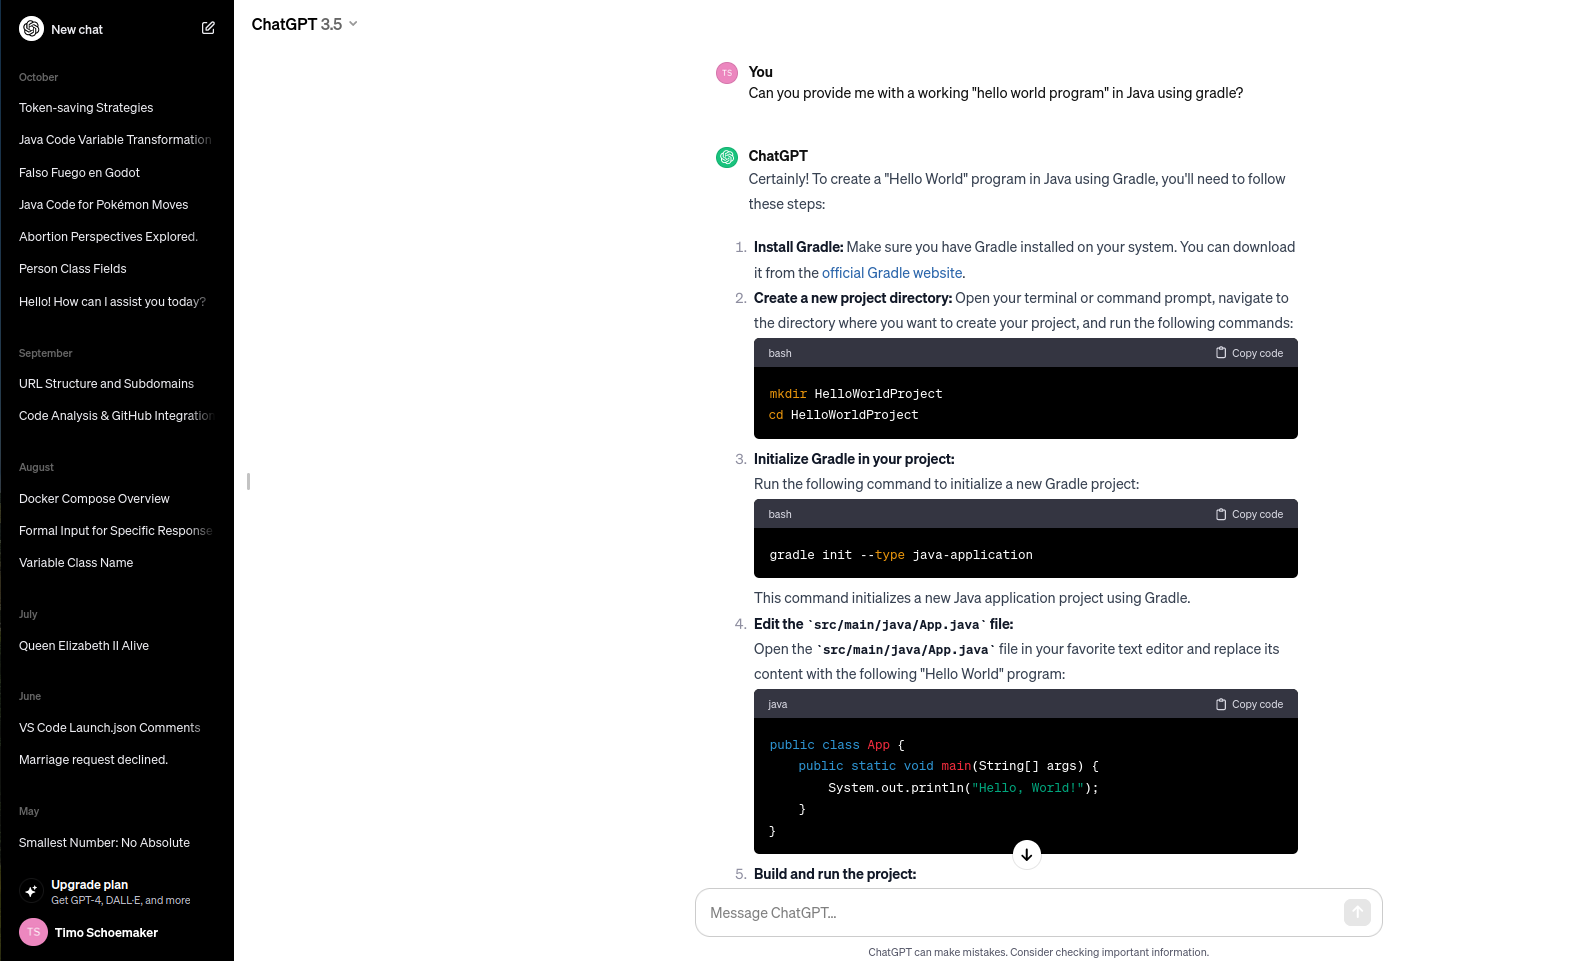
\includegraphics[width=\columnwidth]{figures/chapter2/chatgpt_browser.png}
    \caption{ChatGPT in the browser}
    \label{fig:chatgpt_browser}
\end{figure}
In the main panel that encompasses the most area of the figure, a chat is visualized. This is the the chat with the ChatGPT model. The queries are headlined with \textit{You} and the responses with \textit{ChatGPT}. In this example, ChatGPT is asked to create a \textit{hello world} program with gradle. As a response, the model returned code blocks that the user can simply copy and use. Also descriptions are provided to explain the context and usage of the code.

On the right side, all conversations with ChatGPT are listed. For instance, there is a conversation about \enquote{IntelliJ PSI Modification Fix}. A user can have multiple independent conversations where each has it own context. 

\subsubsection{API}
In order to use the ChatGPT \ac{API}, a user has to create an OpenAI account and deposit financial information so that the user can be charged. Each request to the API consumes a certain amount of tokens dependent on the query. 

A token is the smallest unit used by ChatGPT to process a query. For instance, a token could be one english word, a syntactical part of a programming language, a number, or a similar independent part of a query. According to OpenAI, a token is 3/4 of a word, so 100 tokens are about 75 words. However, this is just an estimate for natural language texts in the English language. 

The \ac{API} itself used JSON combined with \ac{HTTP}. For the purpose of this master thesis, only a subset of the available means to use the \ac{API} will be explained because the whole \ac{API} would be too complex and irrelevant. 

Listing \ref{lst:chatgpt_api} shows how an \ac{API} query may look like if it used via \textit{curl} which is a tool to  perform \ac{HTTP} requests:
 \begin{figure} [htbp!]
			\lstinputlisting
			[caption={ Example query to ChatGPT  \cite{ChatGPT_url} (\textit{Temperature attribute added})}, 
			label={lst:chatgpt_api},
			captionpos=b,language=java, basicstyle=\footnotesize, tabsize=2, showstringspaces=false,  numbers=left]
			{figures/chapter2/chatgpt_api.json}
		\end{figure}
 

Since ChatGPT uses \ac{JSON} for communication, the content header of \ac{HTTP}  must be set to \enquote{application/json} (l. 2). Afterwards a token must be provided to ChatGPT (l. 23). This  token must be generated on the OpenAI website and will be used to connect the query to an OpenAI account so that the user can be charged properly- The token should remain secret and may not be disclosed (e.~g. via \ac{VCS}) 

Then, the actual query is defined (l. 4-24.). Firstly, the model is defined (l. 5). OpenAI provides multiple models that have different advantages and disadvantages. For instance, a newer model like \textit{gpt-4} has more capabilities but is more expensive.  By providing a temperature, a user can configure the randomness of the response (l.6). A higher temperature results in more creative answers but this creativity might worsen the quality. 

Afterward, the actual messages are provided (l. 7-25). Each message is a tuple of a \textbf{role} and a \textbf{content}. The content of a message is the input or output provided to or by ChatGPT. 

The role of a message indicates the source of a message. If the content of the messages comes from a user, the role should be \enquote{user} (l. 13). A reply for a query is defined as the role \enquote{assistant} (l. 17). The system role is a more specific and can be used to include further context for ChatGPT without eliciting a response (l. 9)

The response of the ChatGPT \ac{API} based on listing \ref{lst:chatgpt_api} is displayed in listing \ref{lst:chatgpt_api_response}.
 \begin{figure} [htbp!]
			\lstinputlisting
			[caption={The response from ChatGPT  \cite{ChatGPT_url}},
			label={lst:chatgpt_api_response},
			captionpos=b,language=java, basicstyle=\footnotesize, tabsize=2, showstringspaces=false,  numbers=left]
			{figures/chapter2/chatgpt_api_response.json}
		\end{figure}

In the bottom part of the listing (l. 13-19), meta information is provided. This includes the response generation time (l. 12), the used model for the response (l. 14), an id for the response (l. 13).

In order for clients to calculate the costs of using ChatGPT, each response also includes how many tokens have been used by the prompt (l. 18), by the response (l. 17), and the total number of tokens (l. 19).

In the upper part of the response (l. 1-11), the actual response is provided. The response is an array of so-called choices (l. 2~-~11). Each choice consists of the actual message (l.~ 6-8), which itself consists of the message content (l. 7) and the role of the content (in most cases, this would be \enquote{assistant}).

The \enquote{finish\_reason} indicates how the \ac{LLM} has finished on the prompt. If the value is \enquote{stop}, the prompt was executed without faults so that the response is valid. If the value is \enquote{length}, the output would exceed the maximum token limit, so the output will be incomplete. The value \enquote{content\_filter} indicates that OpenAI censured the requests because it violates the terms of use of OpenAI. \cite{ChatGPT_url}


\subsection{Advantages and Challenges on using Large Language Models}\label{sec:llm_challenges}

While using  \ac{LLM} for refactoring brings many advantages  and possibilities, using \ac{LLM}  successfully can be challenging. The advantages and disadvantages will be discussed in this subsection. A \textbf{traditional algorithm} as used in this section means any manual refactoring algorithm (e.~g.,~ refactoring data clumps by extracting a class, removing and introducing parameters in methods, and updating all references)

\subsubsection{Advantages}

First of all, large language models are very flexible. A normal refactoring algorithm needs to consider many situations. For instance, a traditional algorithm that modifies the method signature in a class might not work on an interface. A large language model does not need to be adapted to all edge cases but often finds a suitable solution to a problem because it is not restricted to a specific refactoring process. \cite{shirafuji2023refactoring}

Additionally, a \ac{LLM} is more similar to a human as it is more  \enquote{creative}. While it is still a computer model and does not win the Turing-Test \cite{turing_test}, a \ac{LLM} can refactor code in a manner more closely as a human being would do. For instance, it can suggest class names that are related to the topic of the class, which a human being would also consider, while traditional algorithms would use placeholder names, concatenation of field names or other simple name construction algorithms. \cite{shirafuji2023refactoring}

Large language models are also extensible. For instance, if another programming language is used, an \ac{LLM} can be easily adapted, while a traditional refactoring approach would require more effort to be language-agnostic.

Moreover, a \ac{LLM} can refactor the code in more ways than instructed. While a model can be specifically instructed to refactor data clumps, it might also correct formatting errors, spelling mistakes, or other code smells. While the focus of this master thesis will be on data clumps, other code smells are important too and might be more serious. Using a  \ac{LLM} allows developers to fix more code smells without developing and testing more tools to refactor multiple code smells. As they are better to understand the context of the code than a traditional algorithm, the quality of the code can therefore be improved. \cite{shirafuji2023refactoring}

Furthermore, \ac{LLM} can adapt to the coding style of the source code. If for instance, the source code used the \enquote{snake\_case} or the \enquote{pascalCase} naming convention, the model can detect this convention and use it for its own refactoring (e.g. creating new methods, variables or classes). A traditional approach would need to be configured for each project to use the right convention so that the generated code might look more artificial as it does not fit to the rest of the code.


\subsubsection{Disadvantages}

First of all \ac{LLM}s are not trustworthy. They are often confident in their answers which nevertheless are wrong. This confidence can often be broken by asking subsequent questions which lead the \ac{LLM} to rethink the answer. however, doing this in an automatic way is challenging. \cite{azaria2023internal}

Additionally, \ac{LLM} use randomness in their answers which means that the same query can result in different replies. The factors influencing the reply are generally not known and should not be assumed. As a result, requirements regarding a specific output format may be ignored by the model so that developers using a \ac{LLM} must always consider how to parse non-adhering output.  \cite{hu2023large}

One issue that many \acp{LLM} share is hallucination. This means that the model generates a response, but does not come to an end. For instance, an \ac{LLM} generating a \ac{JSON} can add more and more \ac{JSON} objects to its response until it has no space left so that it must abruptly stop leaving an invalid \ac{JSON} with no closed braces.  The conditions when such behavior can be observed are unpredictable and should be taken care for. 

Furthermore, \ac{LLM}s are usually black boxes. They do not give hindsight on how they came to a specific reply. While they can explain their reasoning, it is not possible to check the exact thought process.
While a query can consist of multiple parts, conditions, or requirements, a \ac{LLM} will not always adhere to all of these. It may weigh some requirements, ignore other, or interpret them wrongly so that the result is unexpected. A \ac{LLM} may also come to an intermediate result that it will not show at the end even though the intermediate result was correct or requested. Also, no sources of the information is provided. \cite{chen2023instructzero}

Moreover, \ac{LLM}s do not have access to the latest information about a topic. They cannot access external sources like current news and up-to-date documentation. Instead, they employ a so-called cut-off date. Only information before that cut-off date will be used. As of the time of writing this section, the cut-off date for ChatGPT is April  2023. However, the release was several months later.  

There are also security issues with using  \ac{LLM} like ChatGPT. If a model is asked to generate or refactor code, one cannot trust that the code is safe to use. As a result of the cut-off date, the code might use operations that are considered deprecated or even unsafe to use because security vulnerabilities have been detected in the meantime. As a result, the developer needs to verify whether the code is safe to use which is another burden.  \cite{pearce2021asleep}

Furthermore, it is not out of the question that a malicious attacker might change the query or the reply of a \ac{LLM}. Therefore, using such a model might be a feasible way to hack systems or create damage which is difficult to detect and prevent. \cite{not_what_you_signed_for}

Another significant aspect are the legal implications of using \acp{LLM}. Since these models have only recently become mainstream, there are still unresolved legal issues. For instance, since most \acp{LLM} are trained using publicly available data, there are copyright issues as the idea of a particular line of code might come from somebody unknown. Also there are responsibility questions. What happens if the output of the model is malicious or faulty and who is legally responsible for making sure that no damage is done if the output of a model is used. The answers to these issues depend strongly on the jurisdiction. For instance, in the European Union the EU AI Act (Regulation (EU) 2024/1689), requires  transparency for using \acp{LLM} and bans the use of them in situation critical for human safety.  \cite{eu-ai-act}


Lastly, also costs and capacity considerations needs to be observed. For large projects, a \ac{LLM} might be too costly because  the costs are often dependent on the input size. Therefore, the use of large language models should be adequately prepared so that as many costs as possible can be saved.  \cite{chen2023frugalgpt}




\subsection{Consideration while using large language models}
In order to use a \ac{LLM} more effectively, many considerations should take place beforehand as the quality and potential costs can be strongly affected by them. While an \ac{LLM} can be very flexible and tolerant, ignoring these points nevertheless increases the risk of wrong results. These considerations are  referred to as \textbf{prompt engineering}. Th

\subsubsection{Context window and statelessness}

ChatGPT is stateless. This means that the token id explained above is solely used for accounting purposes and not to store the queries reliably. As a result, if one wants to hold a conversation similar to the browser version,  not only all previous messages from the user must be sent to ChatGPT, but also all replies and messages of the system role. This should be considered while using the OpenAI \ac{API} because the number of required tokens can enormously increase for longer conversations.

\begin{figure}
    \centering
    \includesvg[width=\columnwidth]{figures/chapter2/chatgpt_stateless.drawio.svg}
    \caption{Visualization of statelessness of an \ac{LLM}}
    \label{fig:chatgpt_stateless}
\end{figure}


Figure \ref{fig:chatgpt_stateless} visualize this issue. Here, the user asks the ChatGPT API to find all data clump java files \textit{(request a)}. ChatGPT responds with some data clumps. These might not be all data clumps, so a follow-up request might improve the results \cite{10062688}. Therefore, the user sends another completely new request \textit{(request b)} to instruct the model to find more data clumps. However, ChatGPT responds with a general message stating that no files have been submitted. This is the result of the statelessness which requires that the user always send the whole context with each query. In \textit{request c)}, the context is provided so that ChatGPT accurately responds by finding another data clump.

Since follow-up requests make only sense if ChatGPT has already responded, the whole original request, the reply by ChatGPT, and any previous conversation must be provided which can have a significant impact on costs and rate limits. 

A related issue occurring for some \acp{LLM} other than ChatGPT is the context window. Large language models like ChatGPT can only stores a limited amount of information during a conversation. If the amount of information is too large,  a model can react differently. ChatGPT will throw an error so that the user must reduce the amount of information transmitted to ChatGPT.

Other models will forget some parts of it even though they might be relevant for the use case of the \ac{LLM}.
Assuming, an \ac{LLM} has only a very small context window, which every modern model should easily handle, figure \ref{fig:llm_loose_context} demonstrates the issues that arises  A model is instructed to find and refactor data clumps in java files, and those java files are submitted as well. The response of the model at the bottom of the figure is however unexpected as it only explains the content of the files submitted. The reason for this response is not some misunderstanding of the prompt but a lack of prompt. The transparent rectangle represents the context window, only covering the content of the transmitted files while the instruction is not covered. 
Because of the context window limitation, transmitting the third file overwrites the content of the prompt so that the model forgets the initial instruction and cannot reasonably process the files, giving instead a description of the files. The problem also arises on greater context window if multiple files or large files are involved as it may be the case while refactoring data clumps.

\begin{figure}[ht!]
    \centering
    \includesvg[width=0.6\columnwidth]{figures/chapter2/chatgpt_context_windows_size.drawio.svg}
    \caption{Example of model forgetting context}
    \label{fig:llm_loose_context}
\end{figure}

Also the output size of an \ac{LLM} is often limited. This means that generating larger text, the model might stop suddenly without finishing the text. In most cases, a \enquote{please continue} prompt can instruct the model to finish its response. The output limits are often reached when the model hallucinates. 
\subsubsection{Choosing the right parameters}
When dealing with an \ac{LLM}, a user must configure the model. The most major settings to be configured are the model itself and the temperature.

In this master thesis, the model \textit{gpt-4-1106-preview} is used as it provides a larger context  and output size and supports outputting in \ac{JSON} only. However, the cost associated with this model can be a disadvantages. Alternatively, the model \textit{gpt-3.5-turbo-1106} is cheaper but is not as thoroughly trained. 

The temperature is another import configurable item. Using a higher temperature can be beneficial for creative tasks. On the other hand, the quality can be worse as the outputs can get more unpredictable. 




\subsubsection{Separate instruction and input}
Many queries to \ac{LLM} include an instruction and an input. For instance, a query to find and refactor data clumps could provide the source code containing the possible data clumps \textbf{(input)}. The instruction could be the query \enquote{Find and refactor all data clumps in this source code}. 

OpenAI recommends that the instructions and input be separated as distinctive as possible. It suggests enclosing the input in a block of \textit{"""} or \textit{\#\#\#} to mark what the input and what the instruction is clearly.

\subsubsection{Provide detailed context and how the model should respond}

When generating a reply to a query, a language model will use the available context to process the query and generate an output that attempts to satisfy the user's need. This means that every bit of relevant information can help the language model to generate a better response.

On the contrary, providing irrelevant information can increase the chance of wrong responses, so the creator of a query must always consider what to include in a query and what not. 

In the context of data clump refactoring, the query should include the content of the source code and the programming language. However, files that cannot have data clumps (e.g., configuration files) should not be included.

An instruction for refactoring data clumps should state that only the refactored source code files should be returned without providing explanatory texts or other information, as they can hinder the parsing of the output. 

When using the \enquote{gpt-4-1106-preview} or \enquote{gpt-3.5-turbo-1106} model of the OpenAI-\ac{API}, developers can force the model to respond in \ac{JSON}. Hence, the output can be made more predictable and easier to control. A request using this mode must include the term \enquote{\ac{JSON}}. It should however be noted, that the precise structure of the \ac{JSON} returned may still differ from the request. 


\subsubsection{Chain-of-Thought Prompting}\label{sec:chain of thought}

One way to improve the results from \acp{LLM} like ChatGPT is to separate a query into interconnected sub-queries that lead to a chain of thought. This can be compared to the human thinking process because a human alone tries not to solve a problem at once but breaks it down into simpler problems that are still connected to but easier to solve. \cite{Wei2022ChainOT}

For instance, a query to find and refactor data clumps can be separated into a detection query and a refactoring query. These sub-queries can be further divided into a query for each file or for all files in a single directory. As a result, not one a single query is needed but multiple queries. 

This is useful if a human is reviewing the output from a \ac{LLM} since obvious errors can be spotted more easily if the task is divided into multiple steps. However, it is more challenging for an automated tool since it cannot find errors in the same way. 

Furthermore, one should consider that each queries requires further overhead so that the performance might be impacted more negatively. 




\subsection{Other Large Language Models}

While ChatGPT is the most known \ac{LLM}, there are several alternatives. This section gives only a broad overview as the focus will be on ChatGPT.

Some recent commercial \acp{LLM} services are Claude or Gemini. Compared to ChatGPT, they differ in their training data, context window limitation, or maximum output size. Additionally, their pricing and API usage limits might be more favorable for some users.

A different method  is to use self-hosted \acp{LLM}.
Self-hosting means that the user of a \ac{LLM} has to provide for the infrastructure and resources to run and employ the model. For instance, a separate server could be configured that runs a large language model and listens to requests. This server could be directly set up by the user or rented from another organization (e.g virtual private server). 

With this approach, costs can be saved. Instead of being dependent on the price model of OpenAI which can be subject to changes, the user has to pay for the actual costs (e.g. the monthly rent for a server, the power bills, hardware etc). These might amortize after some years but this is not certain.

Moreover, privacy is more preserved since data does not flow to OpenAI but remains in the control of the user. This is especially important in regions with stricter privacy laws (e.~g. European Union).

A self-hosted \ac{LLM} is also more configurable. There a specific models that have been more intensively trained on coding tasks so that the quality of the results can be improved. The models from OpenAI are more generally trained.  For instance, the \textit{Llama2} model is specialized for human interaction while the \textit{Codellama} is specialized for discussing and generating source code. The \textit{Phind CodeLlama} model is based on the Codellama model and is focused more on the code generation task. 

However, this configuration requires effort and time. Finding a suitable model for a task, installing it, and configuring it is not trivial. For instance, a server needs to be set up that  runs the model, receives queries (e.~g. over a network) and respond back. 

This server must be suitable equipped. In general, at least 32 GB of RAM are necessary. Also video RAM and storage requirements must be met to gain useful performance. These are requirements that cannot be achieved by some users. 




Another problem with self-hosted \acfp{LLM} is that they might have lower standards regarding output control. For instance, generating malicious or illegal content is easier with these models than those from OpenAI as they are more censored. 


Self-hosting \acfp{LLM} should not be confused with self-trained \acp{LLM}. In the latter case, a user must train its own model which requires extensive amount of data, even more processing power and the need to properly design the training process to prevent typical issues of machine learning like over-fitting.
\begin{comment}
\subsubsection{Hosting a large language server}

One method to host a \ac{LLM} is via \textit{Ollama} \cite{ollama}. Ollama is a program to download, configure, and host a local \ac{LLM}. Users can set up a large language model with one command and query the model via the command line or a \ac{HTTP} interface.



After a model has been downloaded, a user can execute the command \textit{ollama run <model>} to submit queries 

Similar to to ChatGPT, there is an \ac{API} to integrate Ollama in other application. After installed, Ollama listens to \ac{HTTP} connections  on localhost and port 11434.

Listing \ref{lst:ollama_request} shows how such an \ac{API} can be used via \textit{curl}.

The difference to the ChatGPT \ac{API} are scarce. In contrast to ChatGPT, there is no header for an authorization token because no direct payment to any organization is needed. 

Additionally, Ollama streams replies by default meaning that not the full response is returned at once but multiple response parts that must be aggregated by the user. As this is not useful in the context of this master thesis, it is disabled by setting stream to false (l. 11).

Moreover, another model is used (l.~4) as the ChatGPT models are not available. 


 \begin{figure} [htbp!]. 
			\lstinputlisting
			[caption={ Example query to ChatGPT  \cite{ChatGPT_url}},
			label={lst:ollama_request},
			captionpos=b,language=json, basicstyle=\footnotesize, tabsize=2, showstringspaces=false,  numbers=left]
			{figures/chapter2/ollama/ollama_request}
		\end{figure}

  \end{comment}